\documentclass{article}
\usepackage[utf8]{inputenc}
\usepackage{enumitem}
\usepackage{amsmath}
\usepackage{mathtools}
\usepackage{amsfonts}
\DeclarePairedDelimiter\ceil{\lceil}{\rceil}
\DeclarePairedDelimiter\floor{\lfloor}{\rfloor}
\newcommand*\xor{\mathbin{\oplus}}
\usepackage[table,xcdraw]{xcolor}
\usepackage{graphicx}
\usepackage{float}
\usepackage{amssymb}
\usepackage{adjustbox}
\usepackage[a4paper,margin=1in,footskip=0.25in]{geometry}
\newcommand{\xmod}[1]{\left(\bmod\ #1\right)}
\newcommand{\ximplies}{\Rightarrow\,}
\newcommand{\ncproblem}[1]{\subsection*{Problem #1}}
\newcommand{\problem}[1]{\clearpage\subsection*{Problem #1}}
\newcommand{\xbf}[1]{\mathbf{#1}}
\newcommand{\xbb}[1]{\mathbb{#1}}
\newcommand{\oa}[1]{\overrightarrow{#1}}
\newcommand{\pd}[1]{\frac{\partial}{\partial #1}}

\title{\huge{Generative Adversarial Urban Growth Prediction}}
\author{Ziad Khattab}
\date{}

\begin{document}

\maketitle

\section{Network model}

Prediction of urban growth from a sequence of satellite images requires not only the identification of growth patterns, but the ability to generate images of future maps with decently realistic quality and good enough definition to visually identify urban and non-urban areas. For this, a generative adversarial network (GAN) is used.

In a GAN, a generator network receives the history frames and attempts to provide a realistic continuation to the clip, and a discriminator network attempts to determine whether the clips it receives are real or fake, assigning a probability to the image between 0 and 1 of how likely it is to be real. The two networks compete against one another, with the generator attempting to fool the discriminator into thinking that the generated output images are areal, while the discriminator attempts to pick apart real and fake images more accurately.

\begin{minipage}[t]{\linewidth}
    \centering
    \adjustbox{valign=t}{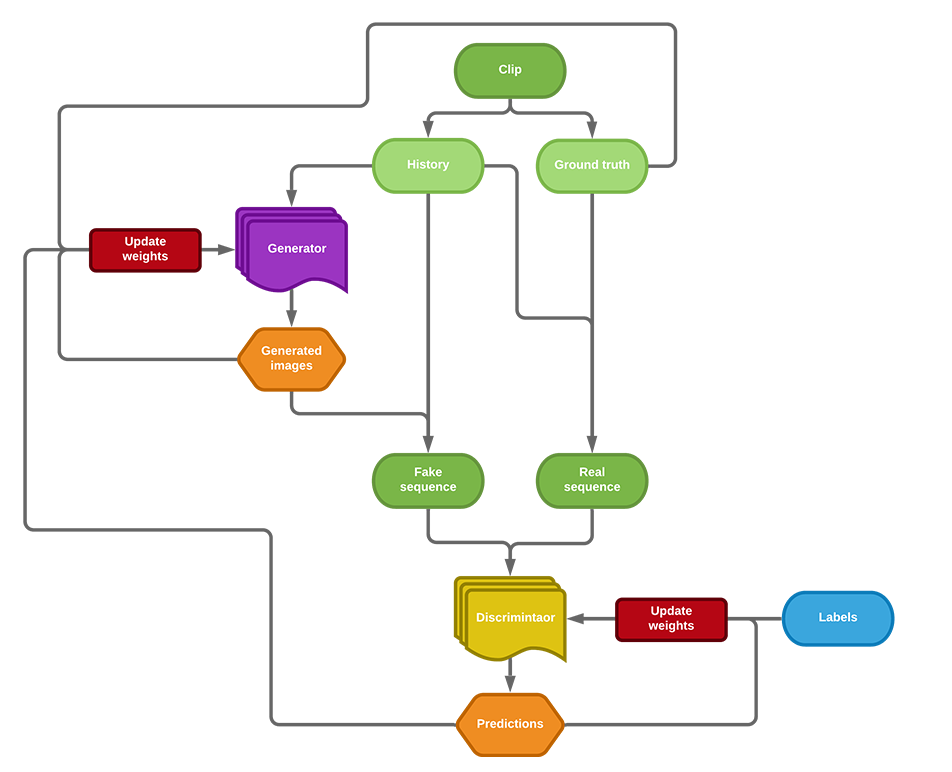
\includegraphics[width=0.8\linewidth]{gan-graph.png}}
\end{minipage}

The discriminator is a convolutional neural network image classifier that runs the clips through convolutional layers activated with ReLU, and then to fully connected layers to obtain a scalar prediction between 0 and 1. It operates on a multi-scale model, meaning that a 48 by 48 pixel square clip is downscaled to 6 by 6, 12 by 12, 24 by 24, and the original clip, and a prediction generated for each scale.

\begin{minipage}[t]{\linewidth}
    \centering
    \adjustbox{valign=t}{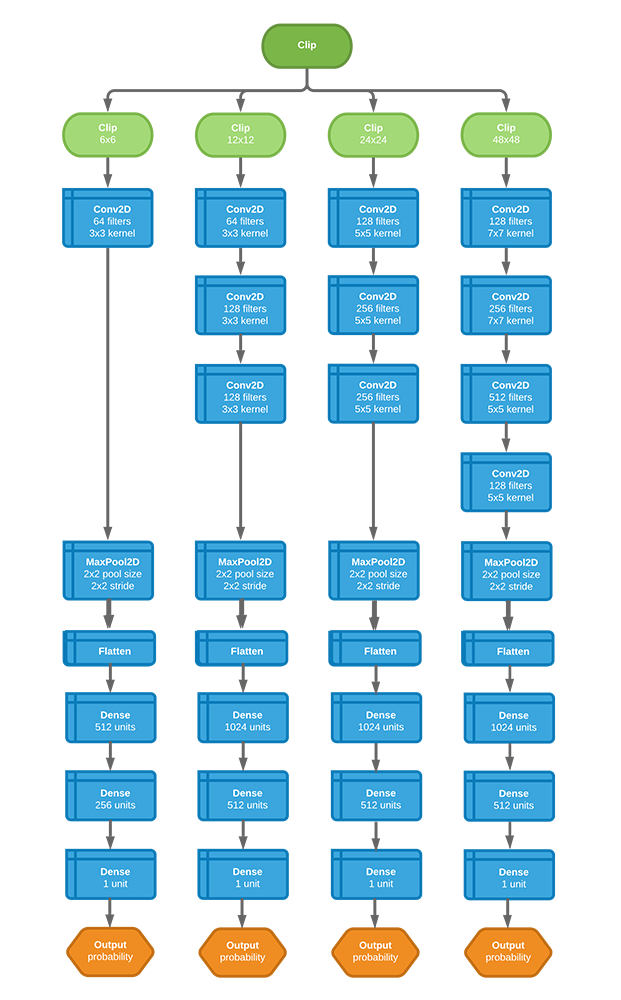
\includegraphics[width=0.85\linewidth]{disc-graph.png}}
\end{minipage}

The generator is a fully convolutional image generator model that also operates with the same four-scale model. However, a significant difference from the discriminator is that the generator concatenates the upsampled output of each scale to the next one to strengthen the time dependency.

\begin{minipage}[t]{\linewidth}
    \centering
    \adjustbox{valign=t}{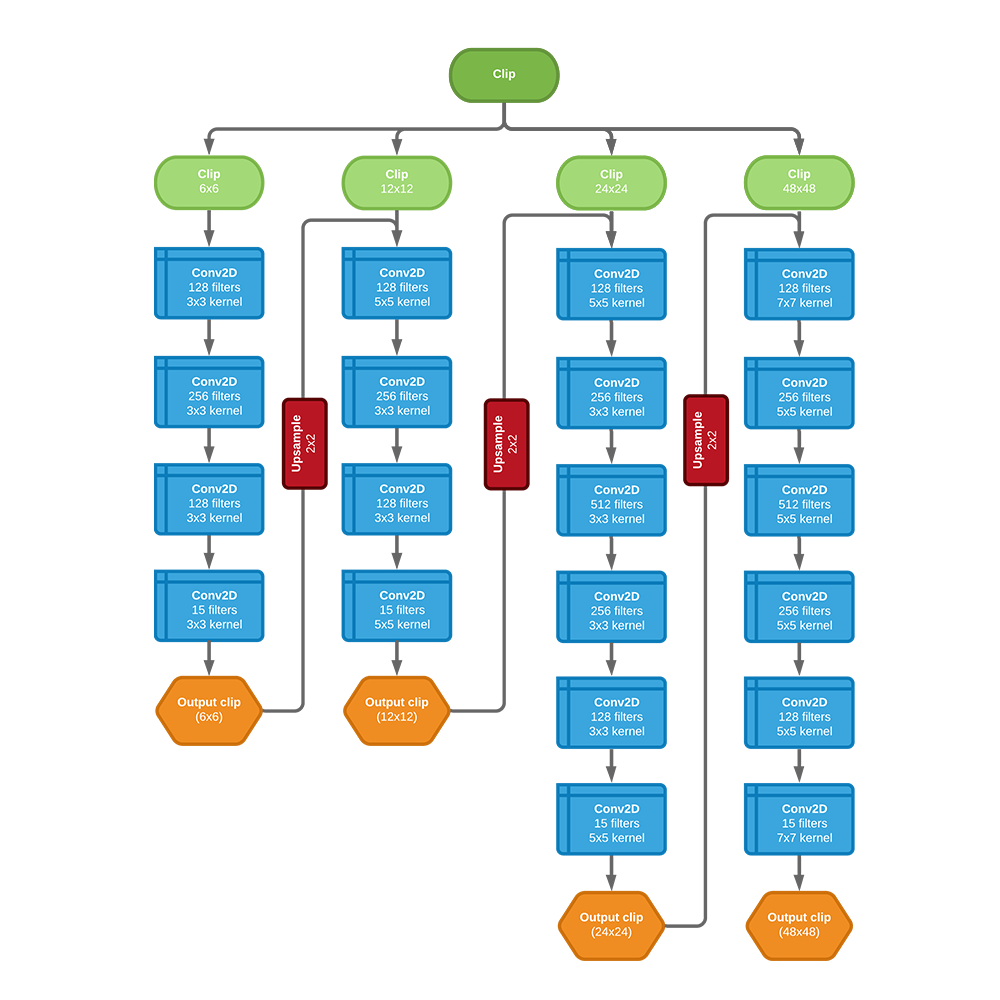
\includegraphics[width=0.8\linewidth]{gen-graph.png}}
\end{minipage}

\end{document}
